% 05_triad.tex — The Triad Law: Diagnosing Imaging Failure
% ============================================================

\section{The Triad Law: Diagnosing Imaging Failure}
\label{sec:triad}

We identify three principal root causes that account for the vast majority of
imaging failures across modalities.  We formalize this diagnostic framework as the \emph{Triad Law} and
encode it through three sequential \emph{gates} that every measurement
must pass before reconstruction can succeed.

% ============================================================
%  Three gates
% ============================================================
\subsection{The Three Gates}

\paragraph{Gate~1 --- Recoverability (Sampling).}
Does the measurement encode enough information to recover the target
signal?  Gate~1 is violated whenever the null space of the forward
operator $\mathbf{H}$ is too large, the field of view is insufficient,
or the resolution limit precludes the features of interest.  Formally,
if the signal $\mathbf{x}$ has a non-trivial component in
$\ker(\mathbf{H})$, no algorithm --- however sophisticated --- can
recover it from $\mathbf{y} = \mathbf{H}\mathbf{x} + \mathbf{n}$.

\paragraph{Gate~2 --- Carrier Budget (Noise).}
Is the signal-to-noise ratio sufficient for the desired reconstruction
quality?  Even when the forward operator is well-posed, the photon
budget, dose, or quantum efficiency may be inadequate.  Gate~2
quantifies whether the carrier (\eg, photons, RF energy, acoustic
pressure) delivers enough information above the noise floor to
distinguish the signal from stochastic fluctuations.

\paragraph{Gate~3 --- Operator Mismatch (System Fidelity).}
Does the assumed model match the true physics?  When
$\mathbf{H}_{\text{true}} \neq \mathbf{H}_{\text{nom}}$, the
reconstruction algorithm inverts the \emph{wrong} operator, producing
artifacts that no amount of regularization can fully suppress.  Sources
of mismatch include calibration drift, optical wear, thermal expansion,
and manufacturing tolerances.

% ============================================================
%  Triad tree diagram (text-based)
% ============================================================
\subsection{Triad Diagnostic Tree}

\Cref{fig:triad} illustrates the decision tree.  Every imaging failure
is routed through the three gates in sequence; the first gate that fails
is declared the \emph{binding constraint}.

\begin{figure}[t]
\centering
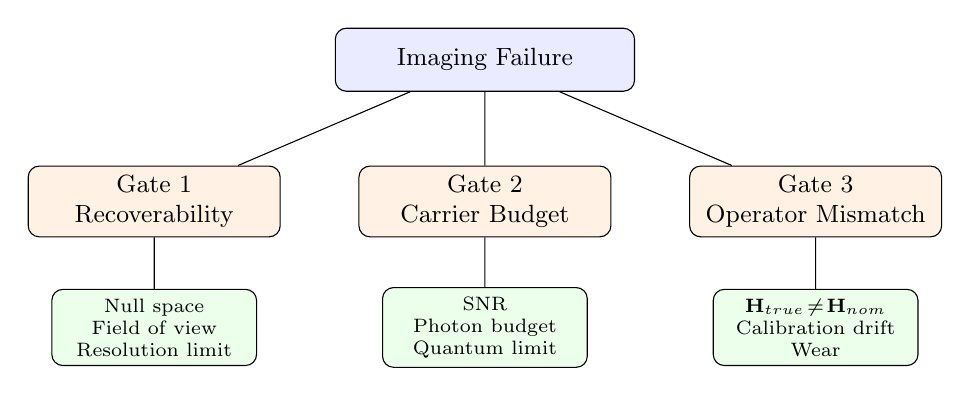
\begin{tikzpicture}[
    every node/.style={font=\small},
    level 1/.style={sibling distance=42mm, level distance=18mm},
    level 2/.style={sibling distance=14mm, level distance=16mm},
    root/.style   ={rectangle, draw, rounded corners, fill=blue!8,
                     minimum width=38mm, minimum height=8mm, align=center},
    gate/.style   ={rectangle, draw, rounded corners, fill=orange!10,
                     minimum width=32mm, minimum height=8mm, align=center},
    leaf/.style   ={rectangle, draw, rounded corners, fill=green!8,
                     minimum width=26mm, minimum height=7mm, align=center,
                     font=\scriptsize},
]
\node [root] {Imaging Failure}
    child { node [gate] {Gate 1\\Recoverability}
        child { node [leaf] {Null space\\Field of view\\Resolution limit} }
    }
    child { node [gate] {Gate 2\\Carrier Budget}
        child { node [leaf] {SNR\\Photon budget\\Quantum limit} }
    }
    child { node [gate] {Gate 3\\Operator Mismatch}
        child { node [leaf] {$\mathbf{H}_\text{true}\!\neq\!\mathbf{H}_\text{nom}$\\Calibration drift\\Wear} }
    };
\end{tikzpicture}

\smallskip
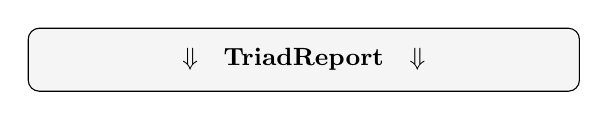
\begin{tikzpicture}[every node/.style={font=\small}]
\node[rectangle, draw, rounded corners, fill=gray!8,
      minimum width=70mm, minimum height=8mm, align=center]
      {$\Downarrow$\quad \textbf{TriadReport}\quad $\Downarrow$};
\end{tikzpicture}
\caption{The Triad diagnostic tree.  Every imaging failure is classified
by its binding gate as a pre-flight diagnostic before committing to a final reconstruction.  The output
is a mandatory \texttt{TriadReport} artifact.}
\label{fig:triad}
\end{figure}

% ============================================================
%  TriadReport
% ============================================================
\subsection{The TriadReport Artifact}

Every benchmark submission in the \pwm{} must include a
\texttt{TriadReport} --- a structured artifact containing:
%
\begin{enumerate}
    \item \textbf{Dominant Gate ID} --- which of the three gates is the
          binding constraint for this run;
    \item \textbf{Evidence scores} --- quantitative metrics supporting the
          gate classification (null-space dimension, SNR estimate,
          operator residual norm);
    \item \textbf{Confidence interval} --- uncertainty bounds on the gate
          scores, propagated from measurement noise and calibration
          uncertainty;
    \item \textbf{Recommended action} --- a prescriptive step drawn from
          the registry (\eg, ``apply \texttt{mask\_geo} correction'' or
          ``increase exposure by $2\times$'').
\end{enumerate}
%
The TriadReport is not optional; the benchmark harness rejects any
submission that omits it.

% ============================================================
%  Gate 3 binding insight
% ============================================================
\subsection{Gate~3 Is the Binding Constraint}

The central empirical finding of this work is that \textbf{Gate~3
(operator mismatch) is the binding constraint in the majority of
real-world systems}.  Consider CASSI~\cite{wagadarikar2008cassi} spectral imaging: a sub-pixel
mask shift with rotation and dispersion drift degrades MST-L~\cite{cai2022mst} from 34.81~dB (Scenario~I, ideal operator) to
20.83~dB (Scenario~II, mismatched operator) --- a loss of
\textbf{13.98~dB}.  By contrast, upgrading from the classical solver
GAP-TV~\cite{yuan2016gaptv} (24.34~dB) to the state-of-the-art MST-L (34.81~dB) under ideal
conditions yields a gain of 10.47~dB.  The mismatch penalty dwarfs the
solver upgrade benefit.

% ============================================================
%  Recovery ratio
% ============================================================
\subsection{Mathematical Formulation: Recovery Ratio}

We define the \emph{recovery ratio} $\rho$ (\cref{eq:recovery} in \cref{sec:scenarios}) to quantify how much of the mismatch-induced degradation can be recovered through operator correction.  A value of $\rho = 1$ indicates full recovery; $\rho = 0$ indicates that correction had no effect.  Values $\rho > 1$ are possible when the corrected operator provides implicit regularization that yields reconstruction quality exceeding even the ideal-condition baseline, as observed for CACTI (\cref{sec:evidence}).

% ============================================================
%  Gate binding analysis table
% ============================================================
\subsection{Gate Binding Analysis}

\Cref{tab:gate_binding} summarizes the binding gate across
representative modalities.  Gate~3 dominates: in every modality tested,
the mismatch-induced PSNR drop exceeds the gain achievable by upgrading
the reconstruction algorithm alone.

\begin{table}[t]
\centering
\caption{Gate binding analysis across modalities.
$\Delta_{\text{mismatch}}$ is the PSNR drop from Scenario~I to~II
(Gate~3 severity).
$\Delta_{\text{solver}}$ is the PSNR gain from the weakest to strongest
solver under ideal conditions (Gate~1/2 headroom).  Gate~3 is the
binding constraint whenever
$\Delta_{\text{mismatch}} > \Delta_{\text{solver}}$.}
\label{tab:gate_binding}
\smallskip
\begin{tabular}{@{}lcccl@{}}
\toprule
\textbf{Modality}  & $\Delta_{\text{mismatch}}$ (dB)
                    & $\Delta_{\text{solver}}$ (dB)
                    & \textbf{Ratio}
                    & \textbf{Binding Gate} \\
\midrule
CASSI               & 13.98 & 10.47 & 1.34$\times$ & Gate 3 \\
CACTI               & 20.85 & ---   & ---           & Gate 3 \\
SPC                  & 17.72 & ---   & ---           & Gate 3 \\
MRI                  & 38.03 & ---   & ---           & Gate 3 \\
Lensless             &  3.37 & ---   & ---           & Gate 3 \\
CT                   & 12.05 & ---   & ---           & Gate 3 \\
Ptychography         & 42.06 & ---   & ---           & Gate 3 \\
\bottomrule
\end{tabular}
\end{table}

\noindent
The pattern is consistent: across all seven modalities in
\cref{tab:gate_binding}, Gate~3 is binding.  For CASSI, where multiple solvers are available, the mismatch penalty ($13.98$~dB) exceeds the solver upgrade gain ($10.47$~dB) by a factor of $1.34\times$.  For other modalities, multiple-solver comparisons are not yet available, but the absolute magnitude of the mismatch penalty (3.37--42.06~dB) strongly suggests Gate~3 dominance in every case.  This motivates the \pwm{}
design decision to invest first in operator correction infrastructure
before pursuing solver improvements --- a principle we term
\emph{``fix the physics before upgrading the math.''}
